% !Mode:: "TeX:UTF-8"
\chapter{分支预测限制预测宽度的改进策略}

本章首先介绍香山第一版架构的取指策略,为什么需要限制分支预测的宽度,过宽的分支预测宽度会对整体设计带来怎样的影响。之后介绍如何通过修改每拍取指的基本单位来限制同一次取指内容中分支指令和跳转指令上限。

\section{香山第一版取指策略}

在香山第一版的设计中,取指pc是按照32Bytes对齐的,也就是低5位都为0,然后每次取指固定取32Bytes的指令数据。由于实现了RISC-V的C扩展,即压缩指令集,RISC-V正常的一条指令 (RVI) 占4个Bytes,而C扩展中规定了许多压缩指令 (RVC),这些压缩指令只有2个Bytes长。

增加了压缩指令之后,会带来一些问题,首先就是分支指令可能会跨行,如图3.1所示,为了便于表示,以一个cache line 8Bytes为例,当然实际设计中一个cache line会大得多。图3.1(a)是不带压缩指令的情况,所有指令都是对齐的,不会出现一条指令在两个cache line中各存一半的现象,但是加入了压缩指令之后就会出现图3.1(b)的这种情况,即由于加入了压缩指令,非压缩的指令无法对齐,就会出现一条非压缩指令被2个相邻的cache line截断的情况。

当出现这种情况时,就会导致最后这条分支指令无法在一个周期内被完整取出,如果这条被截断的指令正好是条分支,也只有等到下一周期取到后半条指令码后才能对它进行预译码操作。

\begin{figure}[htb]
    \centering
    \setlength\tabcolsep{3pt}  % 同一行中的图片间隔
    \vspace{5pt} % 图片上部的空白,如果太小的话,图片顶部会与正文内容十分接近
    \begin{tabular}{ccc}
        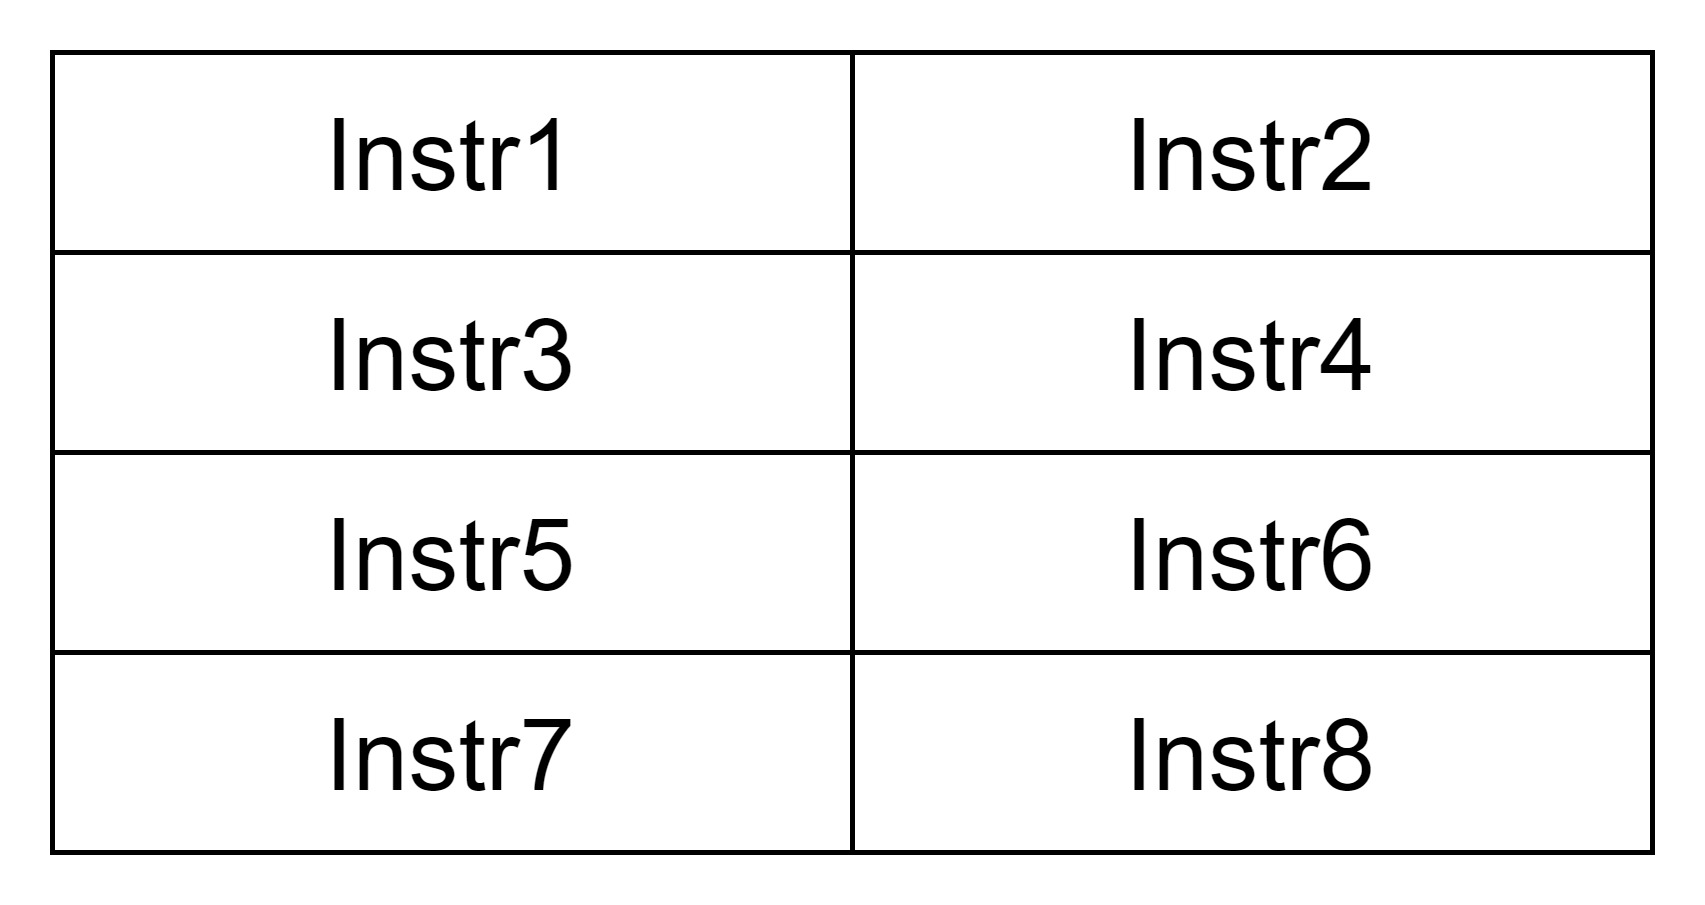
\includegraphics[width=0.30\textwidth]{RVI-only.jpg} &
        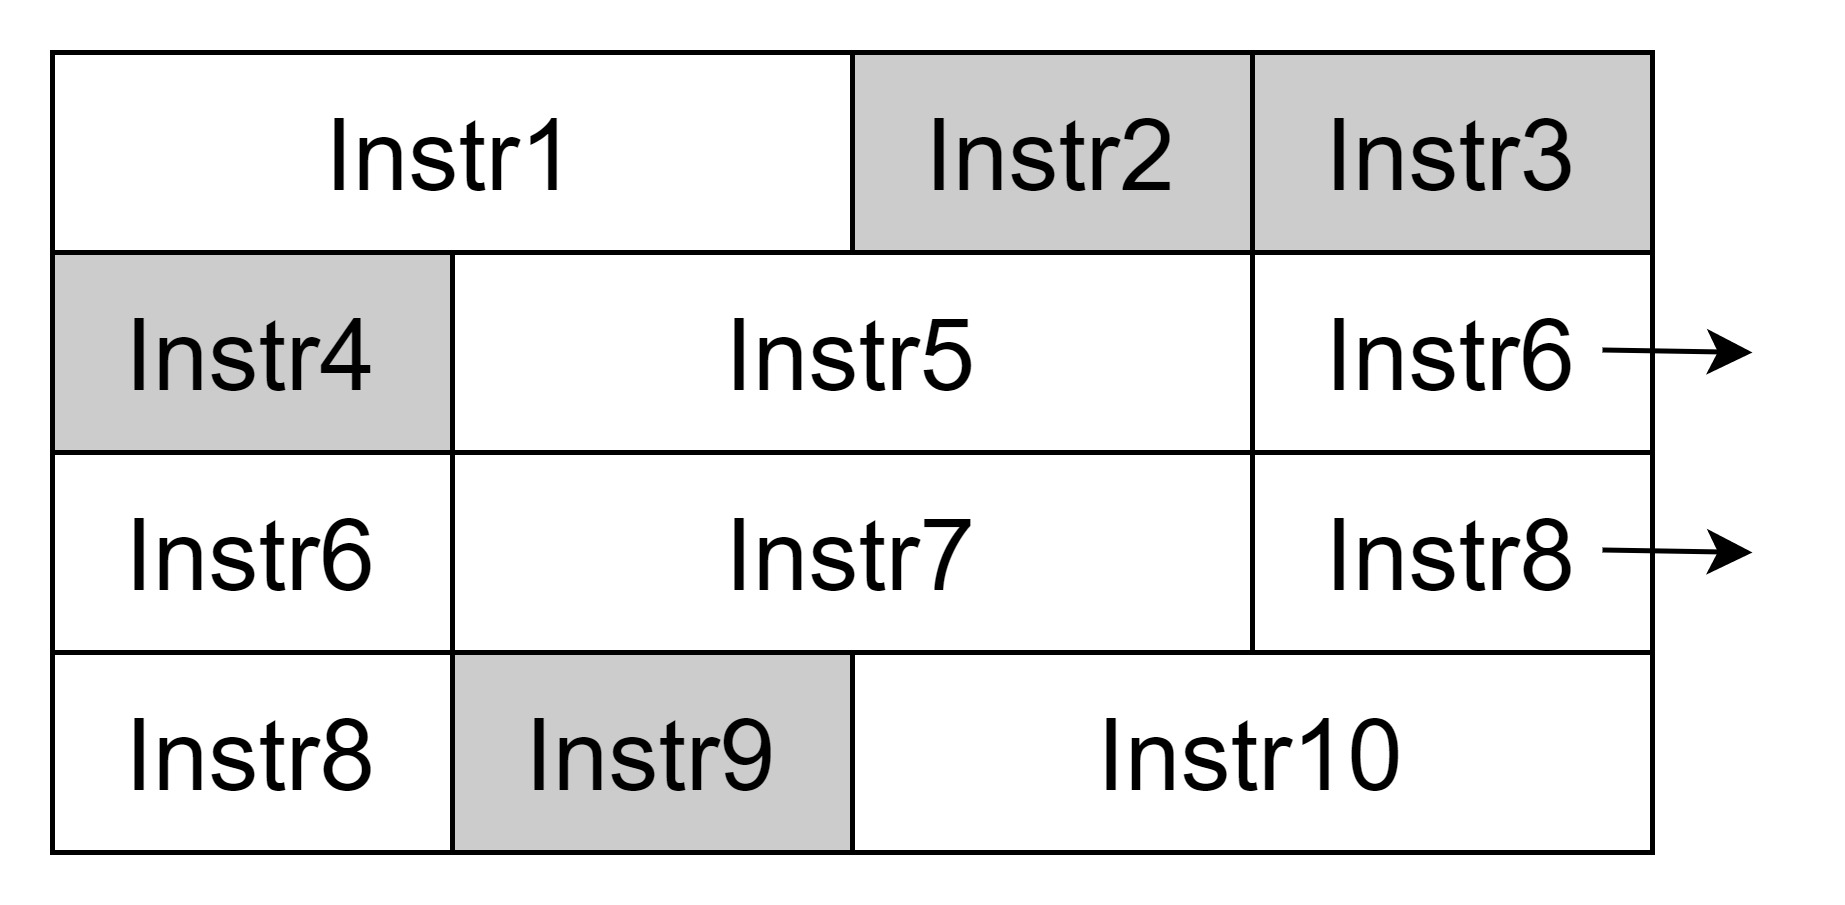
\includegraphics[width=0.325\textwidth]{RVIC.jpg} &
        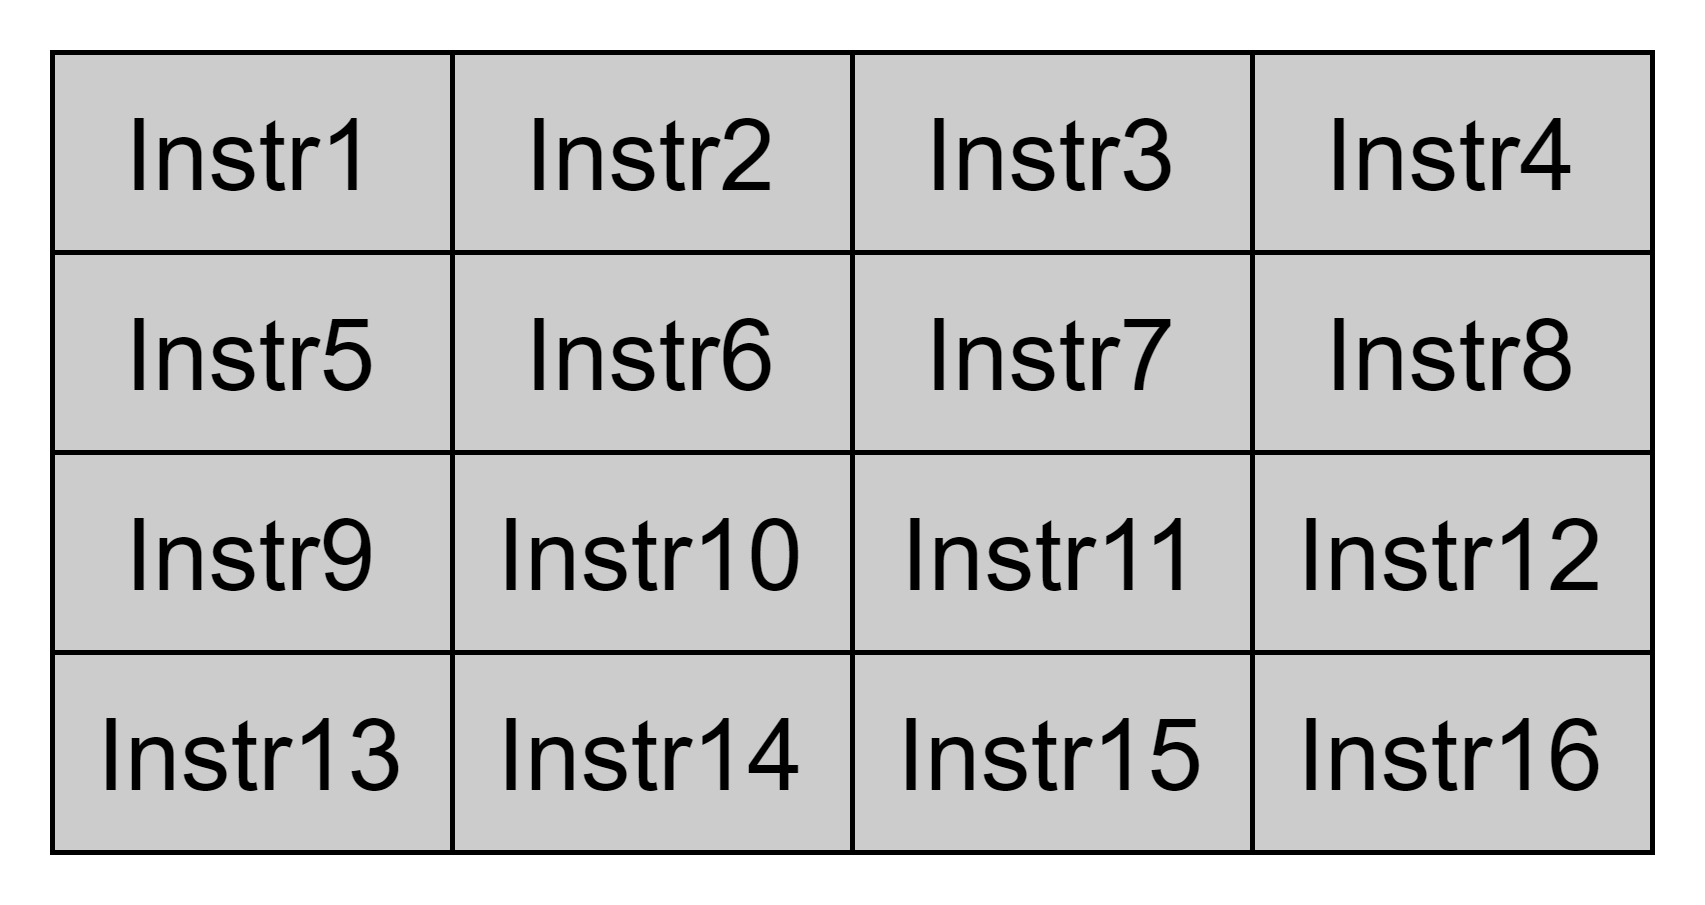
\includegraphics[width=0.30\textwidth]{RVC-only.jpg} \\
        (a) 只有RVI指令 & (b) RVI,RVC指令混合 & (c) 只有RVC指令 \\[1ex]
    \end{tabular}
    \caption{在cache line中以不同形式储存的指令码,其中白色的代表非压缩指令RVI,灰色的代表压缩指令RVC,图(b)中第6和第8条指令跨cache line了}
    \label{fig:figure1}
\end{figure}

加入了压缩指令之后,如果以32Bytes为单位取指,每次取出来的数据中会有8到16条指令不等,最多的情况如图3.1(c)所示,即16条都是压缩指令的情况。因此为了能够覆盖到所有情况,香山第一版的分支预测设计中,所有的预测器,包括第一版中FTB的原型BTB (Branch Barget Buffer) 都是以16为宽度来设计的,也就是说每个预测器都有16个bank,每个bank对应32Bytes中所有有可能是一条分支的位置。

这是一个巨大的开销,这种设计意味着所有的分支预测逻辑的复杂度和连线都会大大增加,尤其是在分支预测最终的时候,我们需要从所有的分支中选出一条最终预测跳转的分支,从16个备选项中选出目标跳转地址,这是一个4级的多选操作,而这个逻辑处于分支预测的很多路径上,是关键路径的一部分,因此降低分支预测宽度,能够减少分支预测的逻辑复杂度,减少最终选择需要的逻辑门数,最终达到优化时序,提高频率的效果。

\section{Fetch Block的定义}

为了降低分支预测宽度,我们需要限制每次取指所能包含的分支指令的最大数量,因为分支预测最终的宽度是以可能的最大分支数量为准的,例如上文提到的如果一次最多会有16条分支,那么分支预测宽度也必须为16,即使大部分时候并没有这么多分支。
假设我们将分支预测的宽度限制为2,之前的取指是以32Bytes定长为单位取指的,而在一些分支指令密集的程序片段中,32Bytes大小的指令块中很大概率会出现超过2条分支,因此我们不能够继续以定长为取指的基本单位,我们需要定义一个新的基本单位,为这个单位添加一些约束条件,以此来限制每次取指的分支指令数量。
我们定义了Fetch Block,

\section{FTB的域设计和管理策略}

投稿论文的主要内容


\section{本章小结}

